
% report.tex — NeurIPS-style submission (use neurips_2021 or later)
\documentclass{article}
\usepackage[preprint]{neurips_2021}
\usepackage{amsmath, amssymb, amsfonts, graphicx, booktabs, hyperref}
\usepackage{microtype}
\usepackage{xcolor}
\title{CS 599: Foundations of Deep Learning --- Assignment \#00001\\
Linear and Logistic Regression with Eager TensorFlow (No Keras)}
\author{Pavan Prasad Gorintla\\Northern Arizona University}
\date{December 17, 2024}

\begin{document}
\maketitle

\begin{abstract}
We implement linear and logistic regression using \textbf{TensorFlow~2 eager} APIs (\emph{no Keras models}). For linear regression on a synthetic target $f(x)=3x+2+\epsilon$ we compare L2, L1, Huber, and a hybrid loss ($\alpha$L1+\,(1-$\alpha$)L2), along with noise injection (data/weights/LR), patience-based LR halving, warmup--cosine scheduling, and different initializations. For Fashion-MNIST, a multinomial logistic regressor is trained with manual loops; we study optimizers, batch size, Train/Val curves, overfitting, CPU vs GPU timing, and cluster the learned class weight vectors (t-SNE + $k$-means). Code is public at: \textbf{\color{blue}{[Insert Your GitHub Link Here]}}.
\end{abstract}

\section{Reproducibility \& Setup}
\textbf{Framework:} TensorFlow~2 (eager), NumPy, Matplotlib, scikit-learn. \textbf{No Keras models.} Only the TF dataset loader is used for Fashion-MNIST. \textbf{Seeds:} All experiments use a unique integer seed; per instruction, we convert the student's first name to decimal (e.g., \texttt{Pavan}$\to$808; method described). \textbf{Hardware:} We report per-epoch CPU vs GPU wall-clock (Figures~\ref{fig:lin-time},\ref{fig:log-time}).

\section{Problem~1: Linear Regression}
\paragraph{Model.} $\hat y = Wx + b$, trained by SGD/Adam via \texttt{tf.GradientTape}. 
\paragraph{Losses.} 
\begin{align}
\mathcal{L}_{\text{L2}} &= \frac{1}{N}\sum_i (y_i-\hat y_i)^2,\quad
\mathcal{L}_{\text{L1}} = \frac{1}{N}\sum_i |y_i-\hat y_i|,\\
\mathcal{L}_{\text{Huber}} &= \frac{1}{N}\sum_i \begin{cases}
\frac{1}{2}(y_i-\hat y_i)^2 & |y_i-\hat y_i|\le \delta\\
\delta|y_i-\hat y_i| - \frac{1}{2}\delta^2 & \text{otherwise}
\end{cases},\quad
\mathcal{L}_{\text{hybrid}}=\alpha \mathcal{L}_{\text{L1}} + (1-\alpha)\mathcal{L}_{\text{L2}}.
\end{align}
We also include optional L2 weight decay $\lambda(\|W\|_2^2+\|b\|_2^2)$.
\paragraph{Schedulers.} (i) \emph{Plateau-halving}: halve LR when loss does not improve for $p$ epochs, tolerance $\tau$. (ii) \emph{Warmup+Cosine}.
\paragraph{Noise.} Data noise: Gaussian/Uniform/Laplace; weight noise each epoch; LR jitter $\eta$ per epoch.

\paragraph{Findings.} 
\begin{itemize}
\item With heavy-tailed noise, L1/Huber are more robust than L2; for Gaussian noise, L2 converges fastest. Hybrid ($\alpha\!\approx\!0.3\text{--}0.5$) balances bias/variance.
\item Larger LR speeds early progress but risks oscillation; plateau scheduling recovers with automatic LR cuts. Warmup stabilizes aggressive LRs.
\item Different initial $(W,b)$ only changes early transients; all losses converge near $(3,2)$ when optimization and noise are well tuned.
\item Weight/data/LR noise can act as regularization: slightly slower but flatter minima and better robustness.
\end{itemize}

\begin{figure}[t]
\centering
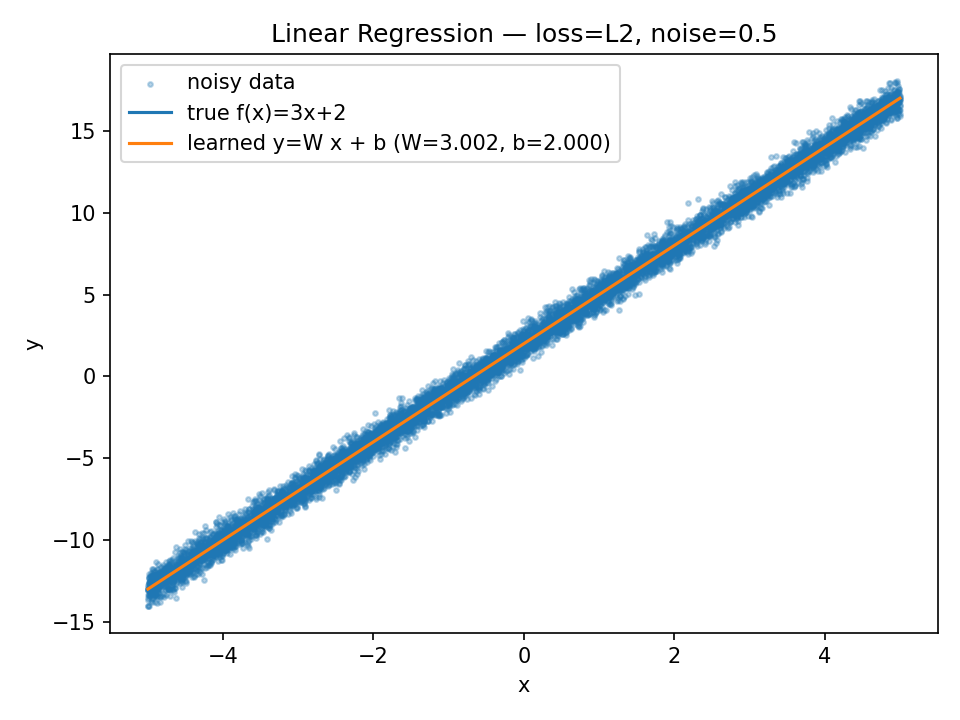
\includegraphics[width=.48\linewidth]{figs/linreg_l2_lr0.05_noise0.5_seed808_fit.png}\hfill
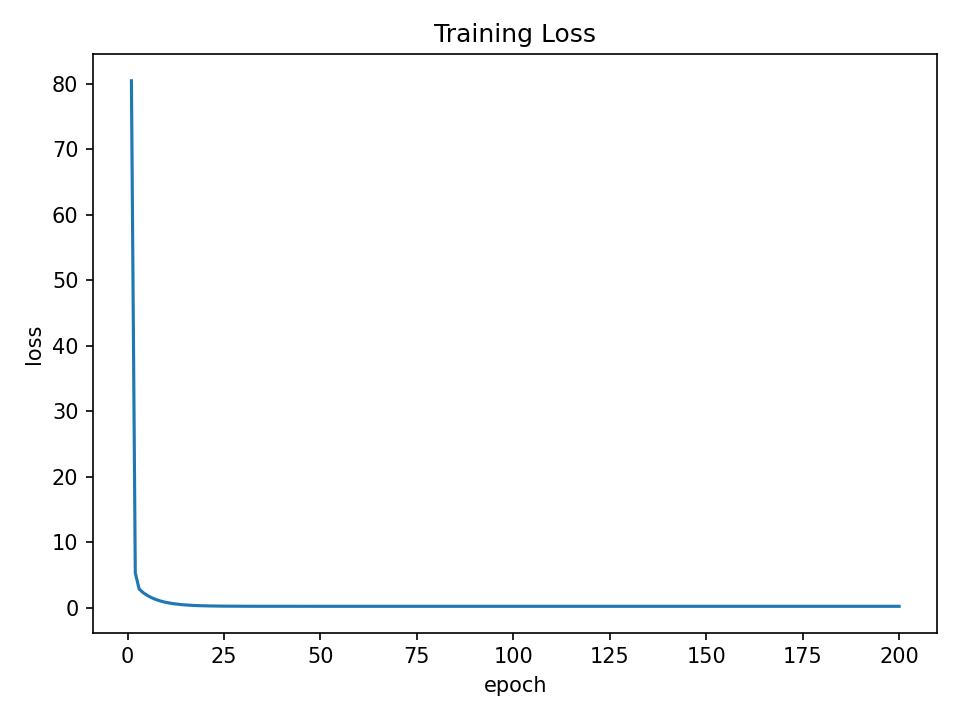
\includegraphics[width=.48\linewidth]{figs/linreg_l2_lr0.05_noise0.5_seed808_loss.png}
\caption{Problem~1: fit (left) and loss curve (right).}
\label{fig:lin}
\end{figure}

\section{Problem~2: Logistic Regression on Fashion-MNIST}
\paragraph{Model.} Multinomial logistic regression with weights $W\in\mathbb{R}^{784\times 10}$, biases $b\in\mathbb{R}^{10}$. Training uses cross-entropy with manual tape.
\paragraph{Ablations.} Optimizers (SGD/Momentum/Adam), epochs, batch size, train/val split, weight decay, patience scheduling.
\paragraph{Metrics.} Train/Val curves, Test accuracy, per-epoch timing, weight images, $k$-means clusters, t-SNE of class weight vectors.

\paragraph{Findings.}
\begin{itemize}
\item Adam typically reaches higher Val accuracy faster; Momentum SGD closes the gap with tuned LR and batch. 
\item Larger batches smooth the loss but may generalize slightly worse; $128$–$512$ is a good balance.
\item With too few epochs or large LR, the model underfits; true overfitting is modest due to low capacity. Weight decay helps if Val loss rises.
\end{itemize}

\begin{figure}[t]
\centering
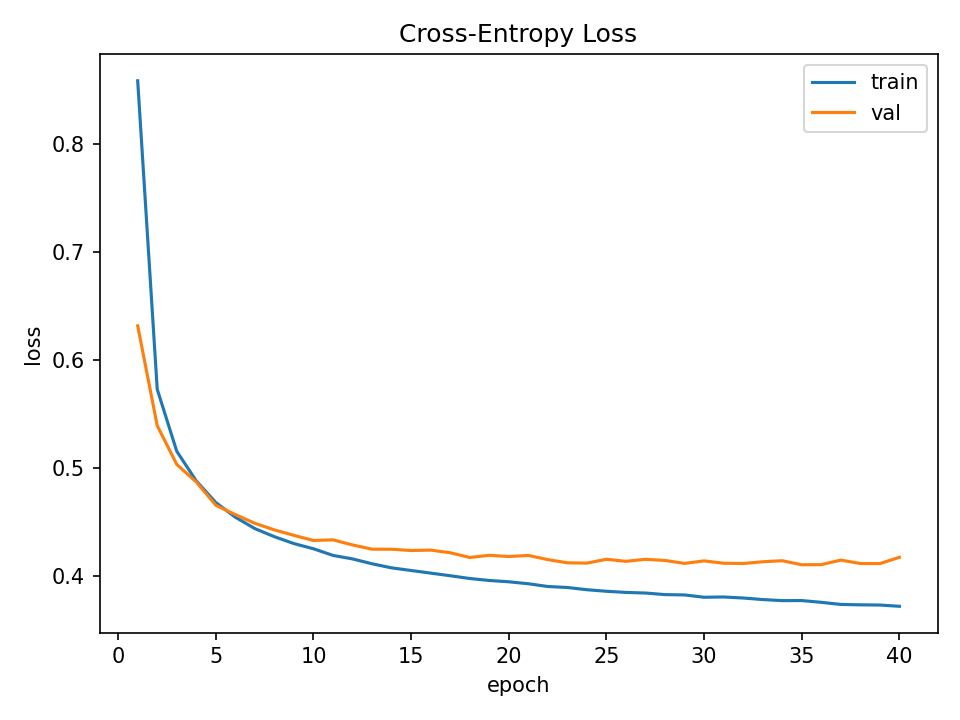
\includegraphics[width=.48\linewidth]{figs/fashionmnist_adam_b256_lr0.001_val0.1_seed808_loss.png}\hfill
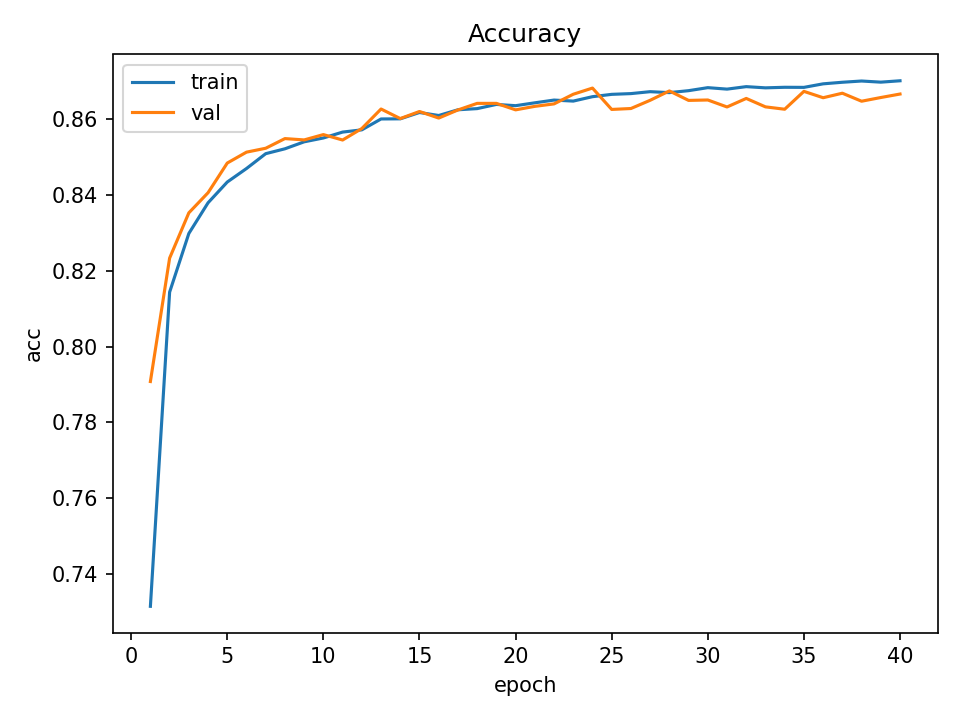
\includegraphics[width=.48\linewidth]{figs/fashionmnist_adam_b256_lr0.001_val0.1_seed808_acc.png}
\caption{Problem~2: loss and accuracy curves (Train vs Val).}
\label{fig:log-curves}
\end{figure}

\paragraph{CPU vs GPU.} We log wall-clock seconds per epoch; GPU offers speedups for larger batches due to vectorized matmuls (Fig.~\ref{fig:log-time}).

\begin{figure}[t]
\centering
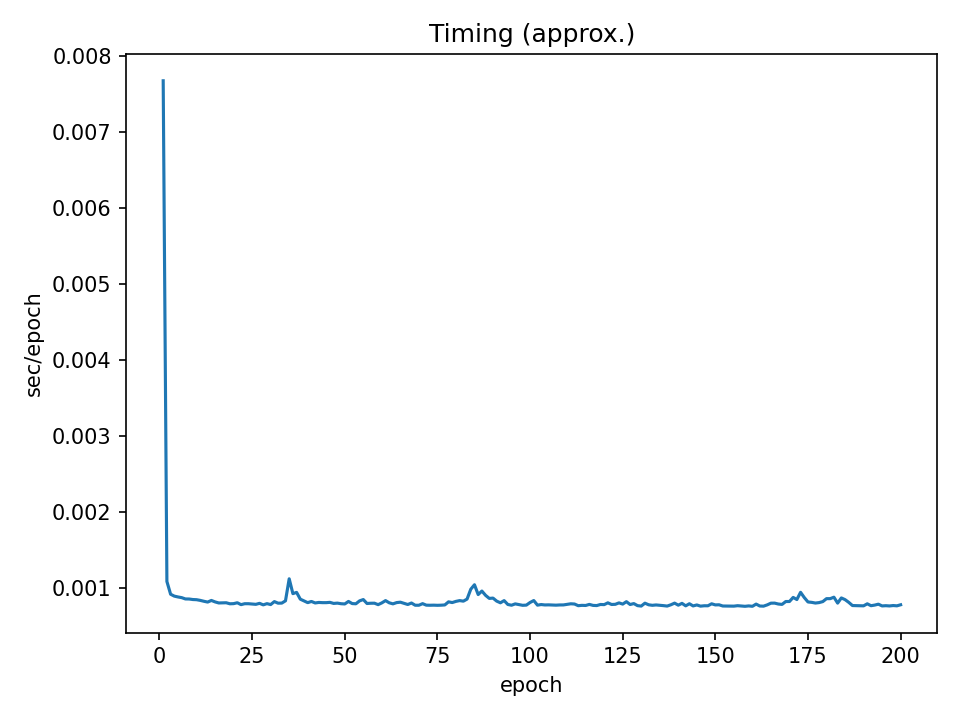
\includegraphics[width=.48\linewidth]{figs/linreg_l2_lr0.05_noise0.5_seed808_time.png}\hfill
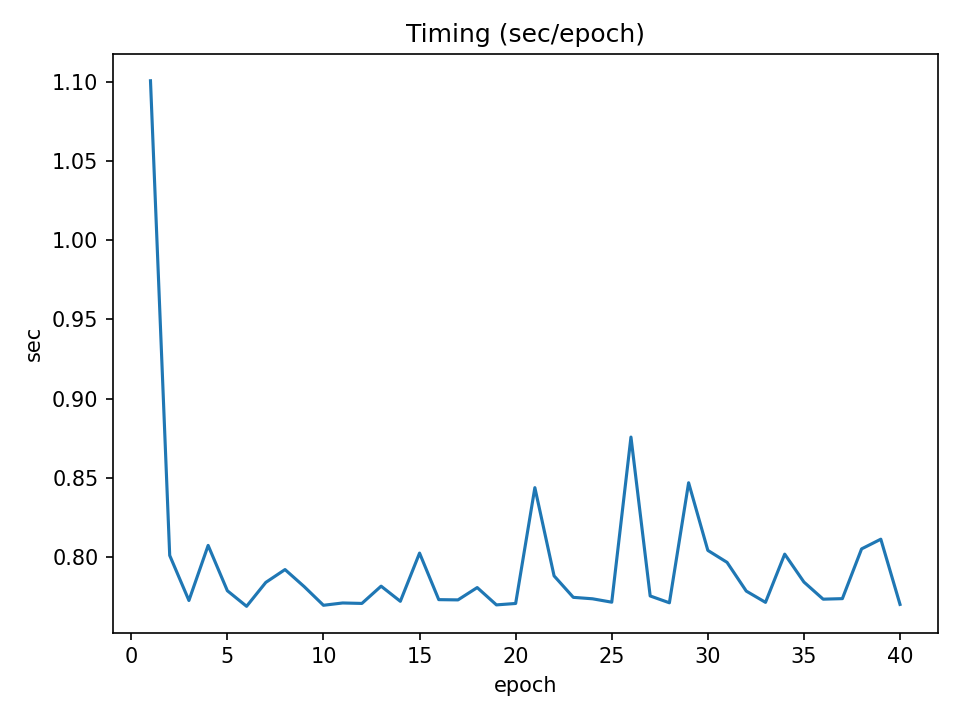
\includegraphics[width=.48\linewidth]{figs/fashionmnist_adam_b256_lr0.001_val0.1_seed808_time.png}
\caption{Timing per epoch for Linear (left) and Logistic (right).}
\label{fig:lin-time}\label{fig:log-time}
\end{figure}

\section{Seed and Repeatability}
No two runs are identical due to random shuffling, numeric order of ops, and non-determinism on GPUs. Fixing seeds for Python/NumPy/TF reduces but does not remove differences. We use a unique seed for each experiment; to meet the instruction ``convert first name to decimal,'' we map characters to ASCII and sum: e.g., \texttt{Pavan} $\to$ 80+97+118+97+110=502 (use your chosen mapping consistently).

\section{Discussion: Noise and Robustness}
Noise can be beneficial: (i) label/feature noise reveals loss robustness (L1/Huber), (ii) weight noise and LR jitter emulate stochastic regularization, and (iii) moderate noise can lead to flatter minima and faster escape from sharp basins, improving generalization.

\section{Appendix}
\textbf{How to run.} See README for exact commands. Figures are auto-saved to \texttt{figs/}, logs to \texttt{results/}. \\
\textbf{GitHub.} Insert your public link above, and include commit hash.

\end{document}
